\section{Chapter 3 - Linear Programming}
\usetikzlibrary{arrows,automata}
\subsection{Tuesday 01/28/2025}
\subsubsection{Linear Tricks}
\textbf{Constraint Relaxation: }
If we have the following optimization problem
\begin{align}
  \text{minimize} & \quad c^\top x \\
  \text{subject to} & \quad \sum_j a_j x_j \leq  b
\end{align},
we can relax the constraint by adding a variable $u$ that will allow us to bend the constraint a bit at a cost.
\begin{align}
  \text{minimize} & \quad c^\top x + cost(u) \\
  \text{subject to} & \quad \sum_j a_j x_j - u \leq b
\end{align}

\textbf{Handling Absolute Values: }
Absolute values can be handled by introducing additional variables and constraints.
One way is to split the variable into a positive and negative component.
\begin{align}
  \text{minimize} & \quad c^\top |x| \\
  \text{subject to} & \quad Ax \leq b
\end{align}
Here, we replace $|x|$ with $x^+ - x^-$
\begin{align}
    \text{minimize} & \quad c^\top (x^+ - x^-) \\
    \text{subject to} & \quad Ax \leq b \\
    & \quad x = x^+ - x^- \\
    & \quad x, x^+, x^- \geq 0
\end{align}

\subsubsection{Example Models}
\textbf{Metabolic Flux Balance: } 
A metabolic flux balance problem is a problem where we have a cell that inputs some nutrient and outputs a metabolic yield, the growth of the cell.
We have a $source$ that is an input into a cell $A$ at a rate $v_1$.
$A$ inputs into $B$ at a rate $v_2$.
In parallel, $A$ inputs into $C$ at a rate $v_3$.
B + C input into $2D$ at a rate $v_4$, etc, the rest of the reaction network model is shown below.
\begin{itemize}
    \item $source \to A \quad (v_1)$
    \item  $A \to B \quad (v_2)$
    \item $A \to C \quad (v_3)$
    \item $B + E \to 2D \quad (v_4)$
    \item $source \to E \quad (v_5)$
    \item $B \to C + F \quad (v_6)$
    \item $C \to D \quad (v_7)$
    \item $D \to biomass \quad (v_8)$
    \item $F \to biomass \quad (v_9)$
\end{itemize}

\begin{center}
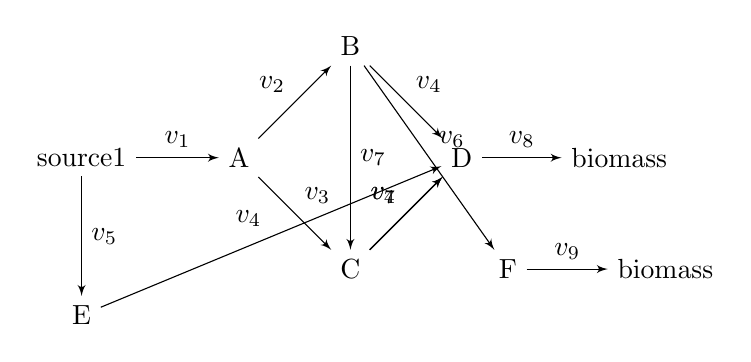
\begin{tikzpicture}[auto, node distance=2cm,>=latex']
    \node [name=source1] {source1};
    \node [right of=source1] (A) {A};
    \node [above right of=A] (B) {B};
    \node [below right of=A] (C) {C};
    \node [below right of=B] (D) {D};
    \node [below of=source1] (E) {E};
    \node [right of=C] (F) {F};
    \node [right of=D] (biomass1) {biomass};
    \node [right of=F] (biomass2) {biomass};

    \draw [->] (source1) -- node {$v_1$} (A);
    \draw [->] (A) -- node {$v_2$} (B);
    \draw [->] (A) -- node {$v_3$} (C);
    \draw [->] (B) -- node {$v_4$} (D);
    \draw [->] (C) -- node {$v_4$} (D);
    \draw [->] (B) -- node {$v_7$} (C);
    \draw [->] (source1) -- node {$v_5$} (E);
    \draw [->] (B) -- node {$v_6$} (F);
    \draw [->] (C) -- node {$v_7$} (D);
    \draw [->] (E) -- node {$v_4$} (D);
    \draw [->] (D) -- node {$v_8$} (biomass1);
    \draw [->] (F) -- node {$v_9$} (biomass2);
\end{tikzpicture}
\end{center}

In this problem, we have an objective we could have multiple goals, one is to maximize the weighted biomass output $w_8 v_8 + w_9 v_9$.
We have constraints that must obey the laws of chemistry and physics. One of them is \textit{mass balance} constraints.
This constraint ensures that the rate of consumption of each edge entering a node is equal to the sum of the rate of production leaving the node.
Flow conservation constraints:
\begin{align}
  \text{maximize} & \quad w_8 v_8 + w_9 v_9 \\
  \text{subject to} & \quad v_1 = v_2 + v_3 \quad (A)\\
  & \quad v_2 = v_4 + v_6 \quad (B)\\
  & \quad v_3 + v_6 = v_7 \quad (C)\\
  & \quad 2v_4 + v_7 = v_8 \quad (D)\\
  & \quad v_5 = v_4 \quad (E)\\
  & \quad v_6 = v_9 \quad (F)
\end{align} 
This problem will be unbounded if we do not constraint the entering sources, so we also introduce \textit{source} constraints.

\textbf{Oil blending}
Consider the problem where we have the following oils with different prices and hardness ratings for each
\begin{itemize}
    \item veg 1 - \$110 - 8.8
    \item veg 2 - \$120 - 6.1
    \item oil 1 - \$130 - 2
    \item oil 2 - \$110 - 4.
    \item oil 3 - \$115 - 5
\end{itemize}
We sell each quantity for \$150.
We have 200 tons of vegetable we can make oil with and 250 tons of non-vegetables we can make oil with.
We want a hardness level between 3 and 6.
To solve this, we can take the vector $\textbf{x} \in \mathbb{R}^5$ as the amount of each liquid $i$ we use. 
We define $\textbf{x}_v$ and $\textbf{x}_n$ subscripts as the subsets of $\textbf{x}$ that are vegetable and non-vegetable.
We similarly define $\textbf{c}$ as the cost vector and $\textbf{h}$ as the hardness vector.
The selling price is $p=150$.
This problem can be formulated as

\begin{align}
  \text{maximize} & \quad 150 (\textbf{1}^\top \textbf{x}) - \textbf{c}^\top \textbf{x} \\
  \text{subject to} & \quad \textbf{1}^\top \textbf{x}_v \leq 200\\
  & \quad \textbf{1}^\top \textbf{x}_n \leq 250 \\
  & \quad 3 (\textbf{1}^\top \textbf{x}) \leq \textbf{h}^\top \textbf{x} \leq 6 (\textbf{1}^\top \textbf{x}) \\
  & \quad \textbf{x} \succeq 0
\end{align}

\subsection{Thursday 01/30/2025}
\subsubsection{Example Models Continued}
\textbf{Oil Blending Over Time}
We now take the oil blending example previously and now consider it over time.
We can buy different raw oil components at different periods of time and store them for use at a later time.
Table \ref{tab:oil_prices} shows the raw oil prices over the next four months
\begin{table}[h!]
\centering
\begin{tabular}{|c|c|c|c|c|c|}
\hline
     & V1  & V2  & O1  & O2  & O3  \\ \hline
M1 & 110 & 120 & 130 & 110 & 115 \\ \hline
M2 & 130 & 130 & 110 & 90  & 115 \\ \hline
M3 & 120 & 110 & 120 & 120 & 125 \\ \hline
M4 & 90  & 100 & 140 & 80  & 135 \\ \hline
\end{tabular}
\caption{Oil prices over time}
\label{tab:oil_prices}
\end{table}

Our storage constraints are that we can store up to 1000 tons of each raw oil each period. 
We start with 500 tons of each oil and must end the total time with 500 tons of each oil.
Going into each period, there is a \$5 cost for holding each ton into the next period.
Our quality constraints are the same, that the total level of hardness must be between 3 and 6. 
Table \ref{tab:oil_hardness} shows the hardness rating of each oil.
Our capacity constraints are that we can not process more than 200 tons of vegetable oil and 250 non-vegetable oil per period. 
\begin{table}[h!]
\centering
\begin{tabular}{|c|c|}
\hline
Oil & Hardness \\ \hline
V1  & 8.8 \\ \hline
V2  & 6.1 \\ \hline
O1  & 2.0 \\ \hline
O2  & 4.2 \\ \hline
O3  & 5.0 \\ \hline
\end{tabular}
\caption{Oil hardness ratings}
\label{tab:oil_hardness}
\end{table}
\\
In order to tackle this problem, we can define the matrix $\Lambda \in \mathbb{R}^{5 \times 5}$  as the cost matrix shown in table \ref{tab:oil_prices}. 
We pad the first row with a 0 vector to represent us starting the first period with inventory.
The matrix $\textbf{X} \in \mathbb{R}^{5 \times 5}$ is our decision variable where each row corresponds to the amount of each oil at the end of each period. 
The first and last column must be equal to a vector of 500s, since we must start and end with 500 of each raw oil.
We also introduce buying and selling variables $\textbf{B} \in \mathbb{R}^{5 \times 5}, \textbf{S} \in \mathbb{R}^{5 \times 5}$ where each row is the amount of an oil we buy and sell before the end of each period.
The first column is $\textbf{0}$ since we can not buy or sell in the 0th period. 
The vector $\textbf{h} \in \mathbb{R}^5$ are the hardness ratings per raw oil.
\\
The buying cost component of the objective function is equal to $\textbf{trace}(\Lambda \textbf{X})$.
The inventory holding cost component of the objective function is equal to $5 (\textbf{1}^\top \textbf{X} \textbf{1} - 500 \times 5)$, the $-500 \times 5$ term is to address the fact that we pay no inventory cost for the 0th period.
The selling component of the objective function is equal to $150(\textbf{1}^\top \textbf{S} \textbf{1})$

\begin{align}
  \Lambda = 
  \begin{bmatrix}
    0 & 0 & 0 & 0 & 0 \\
    110 & 120 & 130 & 110 & 115 \\
    130 & 130 & 110 & 90 & 115 \\
    120 & 110 & 120 & 120 & 125 \\
    90 & 100 & 140 & 80 & 135 \\
  \end{bmatrix}
  \quad
  \textbf{X} = 
  \begin{bmatrix}
    500 & x_{11} & x_{12} & x_{13} & 500 \\
    500 & x_{21} & x_{22} & x_{23} & 500 \\
    500 & x_{31} & x_{32} & x_{33} & 500 \\
    500 & x_{41} & x_{42} & x_{43} & 500 \\
    500 & x_{51} & x_{52} & x_{53} & 500 \\
  \end{bmatrix}
  \\
  \textbf{B} = 
  \begin{bmatrix}
    0 & b_{11} & b_{12} & b_{13} & b_{14} \\
    0 & b_{21} & b_{22} & b_{23} & b_{24} \\
    0 & b_{31} & b_{32} & b_{33} & b_{34} \\
    0 & b_{41} & b_{42} & b_{43} & b_{44} \\
    0 & b_{51} & b_{52} & b_{53} & b_{54} \\
  \end{bmatrix}
  \quad
  \textbf{S} = 
  \begin{bmatrix}
    0 & s_{11} & s_{12} & s_{13} & s_{14} \\
    0 & s_{21} & s_{22} & s_{23} & s_{24} \\
    0 & s_{31} & s_{32} & s_{33} & s_{34} \\
    0 & s_{41} & s_{42} & s_{43} & s_{44} \\
    0 & s_{51} & s_{52} & s_{53} & s_{54} \\
  \end{bmatrix}
\end{align}
\\
The objective function is therefore
\begin{align}
  \text{maximize} & \quad 150(\textbf{1}^\top \textbf{S} \textbf{1}) - \textbf{trace}(\Lambda \textbf{X}) - 5 (\textbf{1}^\top \textbf{X} \textbf{1} - 500 \times 5)
\end{align}

The storage constraints can be expressed as $\textbf{X}_{o,t} \leq 1,000 \quad \forall o \in O, t \in T$. 
Where $O$ is the set of raw oils and $T$ is the set of periods.

The capacity constraints can be modeled as $b_{1t} + b_{2t} \leq 200 \quad \forall t \in T$ and $b_{3t} + b_{4t} + b_{5t} \leq 250 \quad \forall t \in T$.

The hardness constraints can be modeled as $\textbf{S}^\top \textbf{h} \preceq 6 (\textbf{S}^\top \textbf{1}), \textbf{S}^\top \textbf{h} \succeq 3 (\textbf{S}^\top \textbf{1}) $

We also must model our logical inventory constraints that dictate the amount of product we end a period with is equal to the amount we bought during that period, minus the amount we sold, plus the amount we previously had.
$\textbf{X} = \textbf{B} - \textbf{S} + \textbf{X}_{prev}$. Where $\textbf{X}_{prev}$ is a shift of $\textbf{X}$ 
\begin{align}
  \textbf{X}_{prev} = 
  \begin{bmatrix}
    500 & 500 & x_{11} & x_{12} & x_{13} \\
    500 & 500 & x_{21} & x_{22} & x_{23} \\
    500 & 500 & x_{31} & x_{32} & x_{33} \\
    500 & 500 & x_{41} & x_{42} & x_{43} \\
    500 & 500 & x_{51} & x_{52} & x_{53} \\
  \end{bmatrix}
\end{align}

The full optimization problem, with a rather large abuse of different notations and indices can be written as 

\begin{align}
  \text{minimize} & \quad 150(\textbf{1}^\top \textbf{S} \textbf{1}) - \textbf{trace}(\Lambda \textbf{X}) - 5(\textbf{1}^\top \textbf{X} \textbf{1} - 500 \times 5) \\
  \text{subject to} & \quad \textbf{X}_{o, t} \leq 1000 \quad \forall o \in O, t \in T \\
  & \quad \textbf{B}_{1t} + \textbf{B}_{2t} \leq 200 \quad \forall t \in T \\
  & \quad \textbf{B}_{3t} + \textbf{B}_{4t} + \textbf{B}_{5t} \leq 250 \quad \forall t \in T \\
  & \quad \textbf{S}^\top \textbf{h} \preceq 6 (\textbf{S}^\top \textbf{1}), \quad \textbf{S}^\top \textbf{h} \succeq 3 (\textbf{S}^\top \textbf{1}) \\
  & \quad \textbf{X} = \textbf{B} - \textbf{S} + \textbf{X}_{prev} \\
  & \quad \textbf{X}_{o,t}, \textbf{B}_{o,t}, \textbf{S}_{o,t} \geq 0 \quad \forall o \in O, t \in T
\end{align}

\subsection{Tuesday 02/04/2025}

\subsubsection{Standard Form}
Standard form LPs follow the form 
\begin{align}
  \text{minimize} & \quad c^\top x \\
  \text{subject to} & \quad Ax = b \\
  & \quad x \geq 0
\end{align}
we can turn any LP into the above form with some tricks.
An example problem, we want to turn the following optimization problem into standard form
\begin{align}
  \text{maximize} & \quad 3 x_1 + 2 x_2 - x_3 + x_4 \\
  \text{subject to} & \quad x_1 + 2 x_2 + x_3 - x_4 \leq 5 \\
  & \quad -2 x_1 - 2x_4 - x_3 - x_4 \geq 1 \\
  & \quad x_1 \geq 0, x_2 \leq 0 
\end{align}

\begin{align}
  \text{minimize} & \quad -(3 x_1 + 2 (-x_2) - x_3 + x_4)  \\
  \text{subject to} & \quad x_1 + 2 (-x_2) + x_3 - x_4 - s_1 = 5 \\
  & \quad 2 x_1 - 2x_4 - x_3 - x_4 + s_2 = 1 \\
  & \quad x_1, x_2, s_1, s_2 \geq 0
\end{align}
In order to bound variables $x_3, x_4$, we can have them equal $x_3 = x_3^+ - x_3^-$.

\subsubsection{Active Constraints}
Consider the following optimization problem 
\begin{align}
  \text{minimize} & \quad x^2 \\
  \text{subject to} & \quad x \leq 4 \\
  & \quad x \geq -10
\end{align}

\begin{center}
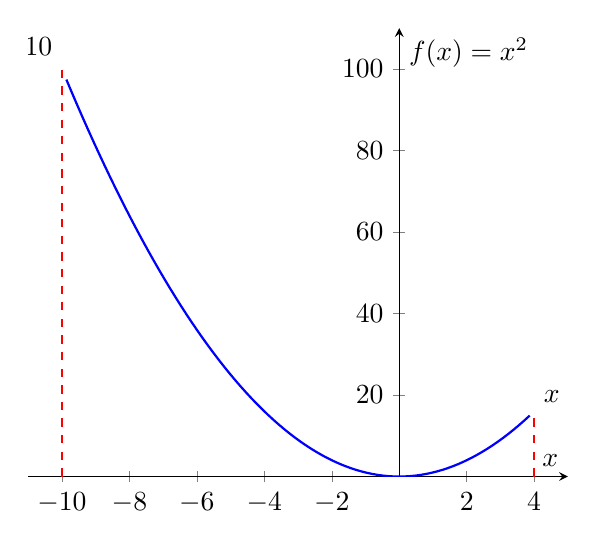
\begin{tikzpicture}
  \begin{axis}[
    axis lines = middle,
    xlabel = $x$,
    ylabel = {$f(x) = x^2$},
    domain=-11:5,
    samples=100,
    ymin=0, ymax=110,
    xmin=-11, xmax=5,
    restrict y to domain=0:110,
    restrict x to domain=-10:4,
    ]
    \addplot [blue, thick] {x^2};
    \addplot [red, thick, dashed] coordinates {(-10,0) (-10,100)};
    \addplot [red, thick, dashed] coordinates {(4,0) (4,16)};
    \node at (axis cs:4,20) [anchor=west] {$x \leq 4$};
    \node at (axis cs:-10,105) [anchor=east] {$x \geq -10$};
  \end{axis}
\end{tikzpicture}
\label{img:quadratic_constrained}
\end{center}
Both of the constraints in the above problem have no effect on the optimal solution.
If they were removed, the answer to the problem would still be the same.
These are inactive constraints.
However, if we consider the next optimization problem
\begin{align}
  \text{minimize} & \quad x^2 \\
  \text{subject to} & \quad x \leq 4 \\
  & \quad x \geq 1
\end{align}

\begin{center}
\begin{tikzpicture}
  \begin{axis}[
    axis lines = middle,
    xlabel = $x$,
    ylabel = {$f(x) = x^2$},
    domain=0:5,
    samples=100,
    ymin=0, ymax=20,
    xmin=0, xmax=5,
    restrict y to domain=0:20,
    restrict x to domain=1:4,
    ]
    \addplot [blue, thick] {x^2};
    \addplot [red, thick, dashed] coordinates {(1,0) (1,1)};
    \addplot [red, thick, dashed] coordinates {(4,0) (4,16)};
    \node at (axis cs:4,17) [anchor=west] {$x \leq 4$};
    \node at (axis cs:1,2) [anchor=east] {$x \geq 1$};
  \end{axis}
\end{tikzpicture}
\end{center}
The optimal solution is at $x=1$.
To formally define an active or inactive constraint, we can use the following:
\\
\textbf{Definition: } Consider $g : \mathbb{R}^m \to \mathbb{R}^p$ and $h : \mathbb{R}^n \to \mathbb{R}^m$.
For $i \in \{ 1, \dots, p \}$inequality constraints,
\begin{equation}
  g_i(x) \leq 0
\end{equation}
is said to be active in $x^*$ if 
\begin{equation}
  g_i(x^*) = 0
\end{equation}
and inactive if 
\begin{equation}
  g_i(x^*) < 0
\end{equation}
The set of indices of active constraints at $x^*$ is deonated as $\mathbb{A}(x^*)$

\subsubsection{Feasible Direction}
Using the same optimization problem as above in \ref{img:quadratic_constrained}, we can illustrate the concept of a feasible direction.
Starting at $x=-10$, the only feasible direction is to proceed in the positive $x$ direction.

For a general optimization problem and a feasible point $x \in \mathbb{R}^n$.
A direction $d$ is said to be feasible in $x$ if there is $\eta > 0$ such that $x + \alpha d$ is feasible for any $0 \leq \alpha \leq \eta$.
Our degree of freedom for movement is one less than the dimension of the total problem. 

\textbf{Theorem: } Let $\mathbb{C}$ be a feasible convex set, and consider $x,y \in \mathbb{C}, y \neq x$.
The direction $d= y-x$ is a feasible direction in $\mathbb{C}$ and $x +\alpha d$ is feasible for any $0 \leq \alpha \leq 1$.

A conclusion that can be drawn from the theorem above is that if we pick an interior point in $\mathbb{C}$ (not on the boundary of $\mathbb{C}$), any direction is feasible.

\textbf{Theorem: } Consider the optimization problem
\begin{align}
  \text{minimize} & \quad f(x) \\
  \text{subject to} & \quad Ax = b \\
  & \quad x \geq 0
\end{align}
and let $x^+$ be a feasible point. 
A direction $d$ is feasible iff $Ad = 0$ and $ d_i \geq 0$ when $x_i^+ = 0$.
\subsubsection{LP Region}
The feasible region for a linear programming problem is a polyhedron.
In canonical form, it can expressed as $\{ x \in \mathbb{R}^n | Ax \leq 0 \}$ and in standard form $ \{ x \in \mathbb{R}^n | Ax = b, x \geq 0 \}$.

\textbf{Vertex: } Let $P$ be a polyhedron. 
A vector $x \in P$ is a vertex of $P$ if it is impossible to find two vectors $y, z \in P, y\neq x, z \neq x$ such that $x$ is a convex combination of the two points.
A convex combination with $0 \leq \lambda \leq 1$ such that
\begin{equation}
  x = \lambda y + (1-\lambda) z
\end{equation}
With this definition of a vertex, we can see that an optimal solution must be at a corner point.

\textbf{Theorem: } Let $P = \{ x \in \mathbb{R}^n | Ax = b, x \geq 0 \}$ be a polyhedron.
$A \in \mathbb{R}^{m \times n}, b \in \mathbb{R}^m$. 
Consider $m$ linearly independent columns of $A$ and the collection of those columns $B \in \mathbb{R}^{m \times m}$ and 
the remaining $n-m$ columns be $N \in \mathbb{R}^{m \times (n-m)}$. 

In order to move around the columns of $A$, we have a permutation matrix $P$.
This permutation matrix has a $1$ in each column and each row.
The permutation matrix will switch around the columns of matrix $A$.
\begin{align}
  AP = 
  \begin{bmatrix}
    B \\
    N
  \end{bmatrix}
\end{align}

\begin{align}
  x = P
  \begin{bmatrix}
     B^{-1} b \\
     0_{n-m}
  \end{bmatrix}
\end{align}
If $B^{-1} b \geq 0$, then this is a vertex
\subsubsection{Basic solution}
Let $P = \{ x \in \mathbb{R}^n | Ax = b, x \geq 0 \}$ be a polyhedron in standard form.
$A \in \mathbb{R}^{m \times n},$ 
$n \geq m,$
$x \in \mathbb{R}^n,$
$ Ax = b$.
This vector $x$ is called a basic solution if 
\begin{itemize}
  \item $B$ is non singular ($B$ is $m$ linearly independent cols of $A$)
  \item $x_i = 0$ if $i \geq m$
  \item x = $B^{-1} b \geq 0$
\end{itemize}

\subsection{Thursday 02/06/2025}
\subsubsection{Basic Feasible Soltuions}
We define the following optimization problem
\begin{align}
  \text{minimize} & \quad c^T x \\
  \text{subject to} & \quad Ax = 0 \\
  & \quad x \geq 0
\end{align}
We have a matrix 
\begin{align}
  A =
  \begin{bmatrix}
     1 & 1 & 1 & 0 \\
     1 & -1 & 0 & 1 
  \end{bmatrix}
\end{align}
We can get a basic solution by picking any two columns of the matrix and creating the basis with those two columns.
We then solve for $x_B = B^{-1} b$ and set the other $x_N = 0$.
A basic solution is the intersection of any two constraints.
A basic feasible solution is the intersection of any two constraints that lie in the feasible region.
By choosing $x_1, x_2$ in the basis from above, we get the following basic solution:
\begin{align}
  \textbf{x} = 
  \begin{bmatrix}
     \textbf{x}_B \\
     \textbf{x}_N
  \end{bmatrix}
  =
  \begin{bmatrix}
    1 \\
    0 \\
    0 \\
    0
  \end{bmatrix}
\end{align}
This solution above has three active constraints and one inactive constraint since $1 > 0$.
This is a basic feasible solution since it obeys the constraints in the original problem.
If we pick $x_2, x_3$ we get the following solution
\begin{align}
  \textbf{x} = 
  \begin{bmatrix}
     \textbf{x}_B \\
     \textbf{x}_N
  \end{bmatrix}
  =
  \begin{bmatrix}
    0 \\
    -1 \\
    2 \\
    0
  \end{bmatrix}
\end{align}
This is a basic solution but is not a basic feasible solution since one of the entries is negative.
Effectively, by finding the basic solutions, we are solving the $Ax = 0$ system and then at the end we check for feasibility against $x \geq 0$.

\subsubsection{LP Solution Analysis}
If all basic variables are $>0$, then we have a unique solution to our problem. 
This is called non-degenerate.
If any basic variables are $=0$, then we have many values of $x$ that will yield the optimal $f^*$.
This is called degenerate.

The simplex algorithm works by traversing these basic solutions.
It traverses along a basic direction.
If $x$ is a basic solution, then a basic direction is a feasible direction along the edges of the polyhedron.

Consider the solution
\begin{align}
  \textbf{x} = 
  \begin{bmatrix}
     \textbf{x}_B \\
     \textbf{x}_N
  \end{bmatrix}
  =
  \begin{bmatrix}
    B^{-1} b \\
    0
  \end{bmatrix}
\end{align},
we want to find a basic direction
\begin{align}
  \textbf{d} = 
  \begin{bmatrix}
     \textbf{d}_B \\
     \textbf{d}_N
  \end{bmatrix}
  =
  \begin{bmatrix}
    d_1 \\
    d_2 \\
    d_m \\
    d_{m+1} \\
    d_{m+2} \\
    d_{n}
  \end{bmatrix}
  =
  \begin{bmatrix}
    d_1 \\
    d_2 \\
    d_m \\
    0 \\
    1 \\
    0
  \end{bmatrix}
\end{align}.
In order to find a basic direction, you set all non-basic variables = 0 except for 1.
We want a feasible direction $d$ where $Ad = 0$.
We can partition $A$ into two matrixes $B,N$.
\begin{align}
  \begin{bmatrix}
     B & N
  \end{bmatrix}
  \begin{bmatrix}
    \textbf{d}_B \\
    \textbf{d}_N
  \end{bmatrix} 
  = B \textbf{d}_B + B \textbf{d}_N
  = 0
\end{align}

We can do some simplification on the middle section as such
\begin{gather}
  = B \textbf{d}_B + B \textbf{d}_N = B \textbf{d}_B + B \sum_{j=m+1}^N A_j d_j \\
  = B \textbf{d}_B + A_p
\end{gather}
Where $A_p$ is the $p$-th column of $A$.

\begin{align}
  \begin{bmatrix}
     a & b & c \\
     d & e & f \\
     g & h & i
  \end{bmatrix}
  \begin{bmatrix}
    \alpha \\
    \beta \\
    \gamma
  \end{bmatrix}
  =
  \begin{bmatrix}
    \alpha a & \beta b & \gamma c \\
    \alpha d & \beta e & \gamma f \\
    \alpha g & \beta h & \gamma i
 \end{bmatrix}
 = \alpha
 \begin{bmatrix}
  a \\
  d \\
  g
 \end{bmatrix}
 + \beta
 \begin{bmatrix}
  b \\
  e \\
  h
 \end{bmatrix}
 + \gamma
 \begin{bmatrix}
  c \\
  f \\
  i
 \end{bmatrix}
\end{align}

Therefore, 
\begin{equation}
  d_B = -B^{-1} A_p
\end{equation}

\begin{align}
  \textbf{d}_p = P
  \begin{bmatrix}
    d_{B_p} \\
    d_{N_p}
  \end{bmatrix}
\end{align}

where $ d_{B_p} = -B^{-1} A_p$ and  $d_{N_p}$ is a basis vector where the $p$-th entry is 1 and the rest are 0.

